% !TEX root = ps2_text.tex

\documentclass[12pt]{article}

% Geometry
\usepackage[a4paper, left=3cm, right=2.5cm, top=2.5cm, bottom=3cm]{geometry}

% Font encoding
\usepackage[utf8]{inputenc} % UTF-8 encoding
\usepackage[T1]{fontenc} % Font encoding
\usepackage{times}

% Math packages
\usepackage{amsmath} % Basic math symbols and environments
\usepackage{amssymb} % Additional math symbols
\usepackage{amsfonts} % Math fonts

% Text packages
\usepackage{parskip}
\setlength{\parskip}{1em}
\usepackage{hyperref}
\hypersetup{
    colorlinks=true,
    linkcolor=blue,
}

% Pictures
\usepackage{graphicx}
\usepackage{float}

% Lists
\usepackage{enumitem}
\setlist[itemize]{itemsep = -0.5em, topsep = -0.5em}

% Bibliography
%\usepackage{cite}

% Loops:
\usepackage{pgffor}

% Title and author
\title{Econometrics II - Problem Set 1}
\author{Ricardo Semião e Castro}
\date{05/2024}


\begin{document}

\maketitle


\section*{Question 1}

\subsection*{Item 1.}
For the process:

$$
Y_{t+s} = \alpha + \delta(t+s) + \epsilon_{t+s} + \theta \epsilon_{t+s-1}
$$

We have:

\begin{align*}
    \frac{Y_{t+0}}{\epsilon_{t}} &= 1\\
    \frac{Y_{t+1}}{\epsilon_{t}} &= \theta\\
    \frac{Y_{t+s}}{\epsilon_{t}} &= 0,~ \forall s \geq 2\\
\end{align*}


\subsection*{Item 2.}

Lets rewrite the process as:

$$
Y_{t} = \delta + Y_{t-1} + \epsilon_{t}\\
Y_{t} = \delta + \sum_{i=1}^{t-1}\delta + \sum_{i=1}^{t}\epsilon_{i}\\
Y_{t} = \delta t + \sum_{i=1}^{t}\epsilon_{i}\\
Y_{t+s} = \delta (t+s) + \sum_{i=1}^{t+s}\epsilon_{i}
$$

We have:

\begin{align*}
    \frac{Y_{t+0}}{\epsilon_{t}} &= 1\\
    \frac{Y_{t+1}}{\epsilon_{t}} &= 1\\
    \frac{Y_{t+s}}{\epsilon_{t}} &= 1,~ \forall s\\
\end{align*}


\subsection*{Item 3.}
In the first case, a $I(0)$ process, the effect of the shock disappeared after two periods -- as $\frac{Y_{t+s}}{\epsilon_{t}} = 0,~ \forall s \geq 2$ --, which can be interpreted as the process having 'low' memory.

In the second case, a $I(1)$ process, the effect of the shock is permanent -- as $\frac{Y_{t+s}}{\epsilon_{t}} = 1,~ \forall s$ --, which can be interpreted as the process having 'high' memory. Regardless of the period, the effect of the shock is always present.



\section*{Question 2}

\subsection*{Item 1. and 2.}
Check the code in the file \textit{ps2\_main.R}. The results are:

\begin{itemize}
    \item For a specification with $5$ degrees of freedom, the rejection rate of the test is approximately $0.1041$.
    \item For a specification with $1$ degrees of freedom, the rejection rate of the test is approximately $0.0876$.
\end{itemize}


\subsection*{Item 3.}

Yes, the results are very different. Specially, the first distribution seems to be in line with the convergence in distribution result aforementioned, while the second is not.

One possible explanation lies in the requirements for such asymptotic result to be valid. In the derivation of the convergence, it was used the "Theorem 1", which stated that the covariance matrix of the bias of the OLS estimators for a deterministic time trend model (multiplied by a scaling in $T$) converged to a well defined matrix only if: $E[\epsilon_t] = 0$, $E[\epsilon^2_t] = \sigma^2$, and  $E[\epsilon^4_t] = < \infty$.

We know that the variance of a t-student RV is $\frac{df}{df-2}$, and it is not well defined if $0 < df \leq 1$. The kurtosis is also not well defined for $0 < df \leq 2$. Thus, the requirements for the mentioned result are not met in the first case, which could explain the difference in the results.



\section*{Question 3}

\subsection*{Item 1.}

\subsection*{Item 2.}

\subsection*{Item 3.}



\section*{Question 4}

First of all, we can plot the historic values and the auto-correlation of the series, to see that it has a clear positive tendency, and a lot of memory. These are signs that indicate a possible unit root.

\begin{figure}[H]
    \centering
    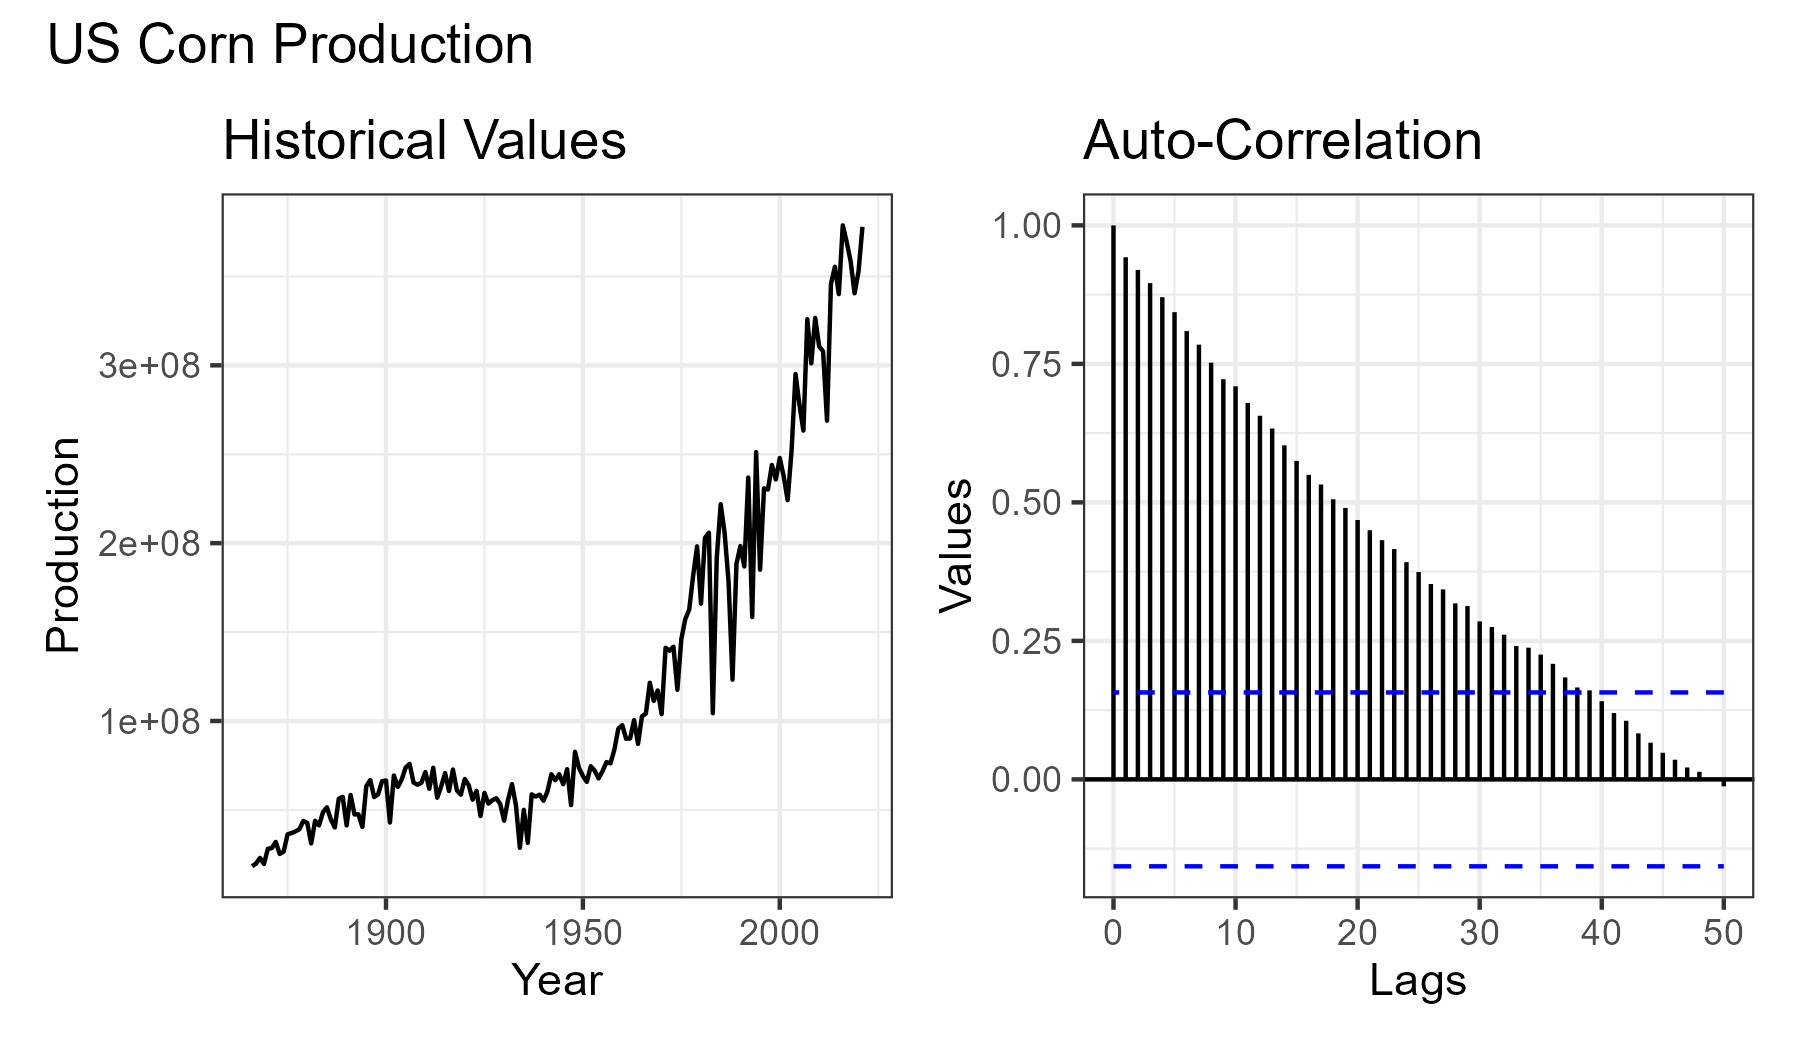
\includegraphics[width=0.8\textwidth]{figures/corn_prod.png}
\end{figure}

Now for the test, we use the function \href{https://rdrr.io/cran/aTSA/man/adf.test.html}{aTSA::adf.test}, that tests three specifications:

\begin{itemize}
    \item Type 1: A linear model with no drift nor linear trend.
    \item Type 2: A linear model with drift but no linear trend.
    \item Type 3: A linear model with drift and linear trend.
\end{itemize}

Each of them with a multitude of lags of the first difference of the serie. In our case, I set the maximum number of lags to 4, given the yearly nature of the data.

Test statistic is the estimated coefficient of the lagged time serie, divided by its standard error. The null hypothesis is that the coefficient is equal to zero, which would indicate an $I(0)$ process.

The results are presented below, with p-values in parenthesis. We can see that the null hypothesis is rejected for all three specifications, for any number of lags, which indicates that the series has a unit root.


% Table created by stargazer v.5.2.3 by Marek Hlavac, Social Policy Institute. E-mail: marek.hlavac at gmail.com
% Date and time: sáb, mai 18, 2024 - 17:42:28
\begin{table}[!htbp] \centering 
  \caption{} 
  \label{} 
\begin{tabular}{@{\extracolsep{5pt}} cccc} 
\\[-1.8ex]\hline 
\hline \\[-1.8ex] 
Lag & Type 1 & Type 2 & Type 3 \\ 
\hline \\[-1.8ex] 
0 & 0.61
(0.82) & -0.54
(0.86) & -2.74
(0.27) \\ 
1 & 2.08
(0.99) & 0.78
(0.99) & -1.16
(0.91) \\ 
2 & 3.01
(0.99) & 1.51
(0.99) & -0.53
(0.98) \\ 
3 & 3.91
(0.99) & 2.21
(0.99) & 0
(0.99) \\ 
4 & 4.87
(0.99) & 3.05
(0.99) & 0.54
(0.99) \\ 
\hline \\[-1.8ex] 
\end{tabular} 
\end{table} 



\end{document}
